	
	


%%%%%%%%%%%%%%%%%%%%%%%%%%%%%%%%%%%%%%%%%%%%%%%%%%%%%%%%%%%%%%%%%%%%%%%%%%%%%%%%%%%%%%%%%%%%%%%%%%%%%%%%%
%%%%%%%%%%%%%%%%%%%%%%%%%%%%%%%%%%%%%%%%%%%%%%%%%%%%%%%%%%%%%%%%%%%%%%%%%%%%%%%%%%%%%%%%%%%%%%%%%%%%%%%%%

\fancychapter{Evaluation}

In this chapter, it will be evaluated the performance gain from each of the main contributions of this work, culminating with the complete multi-threaded version. The results obtained from each benchmark against the relevant comparable software, HMMER's Farrar-based ViterbiFilter vectorization, will be presented and discussed.

\section{Evaluation Methodology}

This section will describe the evaluation methodology and configuration used for the various tests, as well as the features being evaluated. 

\subsection{Benchmark implementations}

As previously described in \sref{hmmer-pipeline}, HMMER uses a multi-level processing pipeline to conduct most sequence homology search tasks. This pipeline is composed by a few filtering levels, each more expensive and fine-grained than the previous one. The current pipeline (HMMER version 3.1b1) has the structure presented earlier in \autoref{figure-hmmer-pipeline1}.

The COPS implementation developed in this thesis targets the second level, as an improvement on the Viterbi Decoding filter of the pipeline. However, the whole pipeline processes the sequences sequentially, one by one, and not in parallel. The multi-threaded parallelization of in HMMER is done by running one different pipeline in each thread. The pipeline itself supports only one thread processing a single sequence.
This pipeline architecture is thus incompatible with both the Rognes method (inter-task vectorization of N concurrent sequences) and the multi-threading developed in COPS (threading of partitions in a wave-front decomposition). 

Given this incompatibility, it was impossible to integrate the developed COPS code into the HMMER pipeline. Instead, the code was packaged into a small stand-alone tool, built on top the HMMER suite. It uses the HMMER libraries and models, and serves as a proof-of-concept for the developed techniques and architecture.

In order to evaluate the overall performance of COPS vis-a-vis the HMMER Viterbi Decoding implementation (i.e., the ViterbiFilter program), a small multi-threaded test tool was created for ViterbiFilter. The benchmark runs with multiple-threads to be fully comparable to the multi-threaded COPS. The used threadpool was implemented efficiently with mutexes and a single synchronized sequence counter.

Besides HMMER's ViterbiFilter, the benchmarks were also run against a serial implementation of Viterbi, optimized for the alignment mode used (Unihit Local alignment).



\subsection{Evaluation Dataset}

To evaluate the developed application, an extensive and thorough range of benchmarks was carried out. The evaluation dataset consists of:

\begin{itemize}

\item HMMs sampled from the Dfam database of Homo Sapiens DNA (\cite{pfam}), with model lengths from 60 to 3000, increasing by a step of roughly 100 model states each time.

Dfam is a widely used database of protein families, and \acp{HMM}s constructed to model them. The latest release of Dfam, as of March 2013, uses HMMER3.1b1 to create the Hidden Markov models. The complete list of chosen HMMs from Dfam is presented below (their length is prefixed to the model name): 

\vspace{1px}
\begin{tabular}{llll}
M0063-U7		& M0700-MER77B			& M1409-MLT1H-int	& M2204-CR1\_Mam	\\
M0101-HY3		& M0804-LTR1E			& M1509-LTR104\_Mam	& M2334-L1M2c\_5end	\\
M0200-MER107	& M0900-MER4D1			& M1597-Tigger6b	& M2434-L1MCa\_5end	\\
M0301-Eulor9A	& M1000-L1MEg2\_5end	& M1727-L1P3\_5end	& M2532-L1MC3\_3end	\\
M0401-MER121	& M1106-L1MD2\_3end		& M1817-REP522		& M2629-L1MC4a\_3end\\
M0500-LTR72B	& M1204-Charlie17b		& M1961-Charlie4	& M2731-Tigger4		\\
M0600-MER4A1	& M1302-HSMAR2			& M2101-L1MEg\_5end	& M2858-Charlie12	\\
				& 						& 					& M2991-HAL1M8		\\
\end{tabular}
\vspace{1px}

\item DNA databases: sequenced genomes of \emph{Homo Sapiens} (Human) and \emph{Macaca Fascicularis} (Crab-eating Macaque), retrieved from the NCBI archive.

\end{itemize}


A wide range of testing configurations were sampled and tried out, to find the best parameters. These tests were mainly described throughout the previous chapter, for instance, the empirical tests to determine the optimal partition length for each target architecture. This extensive testing experience was crucial to tune the parameters for each task requirements, and the overall optimization of the used techniques and implementations. All timings were measured in total walltime, using the Linux \emph{ftime} function.

\begin{table}[H]
\centering
\caption[Hardware details of test machines] {Hardware details of the machines used for the evaluation benchmarks. The No. of cores refers to a single NUMA node}
\label{table-archs}

\begin{tabular}{|c|c|c|c|c|c|c|}
\hline
Spec . Arch.& AMD Bulldozer	& Xeon Nehalem	& i7 Sandy Bridge	\\ \hline
CPU model	& Opteron 6276	& Xeon E7-4830	& i7-3930K 		\\ \hline
Frequency	& 3 GHz			& 2.13 GHz		& 3.20 GHz		\\ \hline
No. cores 	& 8				& 8				& 6				\\ \hline
L1D size	& 16K			& 32K			& 32K			\\ \hline
L1I size	& 64K			& 32K			& 32K			\\ \hline
L2 size		& 2048K			& 256K			& 256K			\\ \hline
L3 size		& 6144K			& 24576K		& 12288K		\\ \hline
\end{tabular}
\end{table}


%As the ViterbiFilter is the second pipeline stage, most sequences are filtered by the first stage (MSVFilter, with computes ungapped local alignments) and never reach the second stage. As such, a realistic dataset should also filter these sequences, and evaluate the Viterbi decoding performance solely with sequences that pass the filter. Therefore, one of the created evaluation datasets (NOME) is composed by the after-MSVfilter sequences from the NRDB90 database, and another dataset from the CHIMP dna.
%=> ha' $\sim$25% das sequencias a passar pelo pipeline ate ao viterbi
%=usando um modelo mais realista (i.e. usei 1a das sequencias da BD como modelo), ficamos com muito mais sequencias que passam na pipeline at? chegar oa viterbi: 26%. 

%=> Podia por o rognes a correr so' com uma thread, q corria as particoes inteiras. Aproveitava a cache na mesma, e dava para usar a paralelizacao da pipeline! tb melhorava o aproveitamento das particoes. MAS era preciso correr as 8 seqs...



\subsection{Evaluation architectures}

The benchmarks were run on three different architectures: AMD Opteron Bulldozer, Intel Xeon Nehalem, and Intel core i7 Sandy Bridge. \autoref{table-archs} presents the detailed characteristics of the hardware used.





\section{Results}

In this section, the benchmark results obtained in the various hardware setups are presented. Each following subsection will focus one of the versions of the developed tool, after each of the main improvements:

\begin{itemize}[noitemsep,topsep=0pt,nolistsep]
\item Inter-task vectorization of the Viterbi algorithm
\item Improved method of loading the Emission scores
\item Partitioning to Model
\item Wave-front multi-threading of the model partitions
\end{itemize}

The benchmarks were all run against the comparable HMMER's vectorized ViterbiFilter. The computing speeds, measured in millions of cells updates per second (a 'cell' corresponds to a state-triplet in HMMs), and the measured speedup against HMMER, will be presented. The serial implementation consistently maintained a constant performance regardless of the model length, so the speedup of COPS against it varied only with the performance of COPS. 


\subsection{Results for the Initial Rognes-based Inter-task vectorization}
\label{Results for the Initial Rognes-based Inter-task vectorization}

\begin{figure}[h!]
    \begin{minipage}{0.48\linewidth}
		\centering
		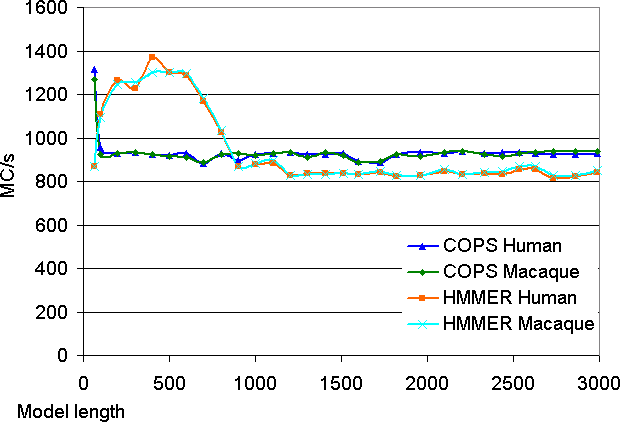
\includegraphics[scale=0.46]{graphics/initial-aleph-runtimes.png}
		\caption[Speeds for the Inter-task vectorization on an AMD Opteron Bulldozer] 
		{Speeds of the initial COPS and HMMER, with the Human and Macaque genomes, on an AMD Opteron Bulldozer.}
		\label{initial-aleph-runtimes}
    \end{minipage}
    \hspace{0.04\linewidth}
    \begin{minipage}{0.48\linewidth}
		\centering
		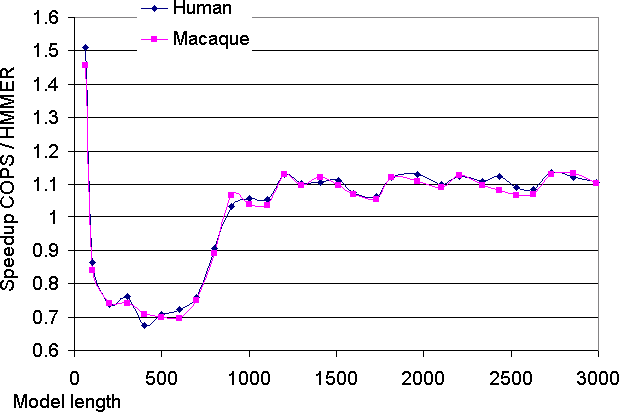
\includegraphics[scale=0.46]{graphics/initial-aleph-speedups.png}
		\caption[Speedups for the Inter-task vectorization on an AMD Opteron Bulldozer] 
		{Speedups of the initial COPS vs HMMER, with the Human and Macaque genomes, on an AMD Opteron Bulldozer.}
		\label{initial-aleph-speedups}
    \end{minipage}
\end{figure} 

\begin{figure}[h!]
    \begin{minipage}{0.48\linewidth}
		\centering
		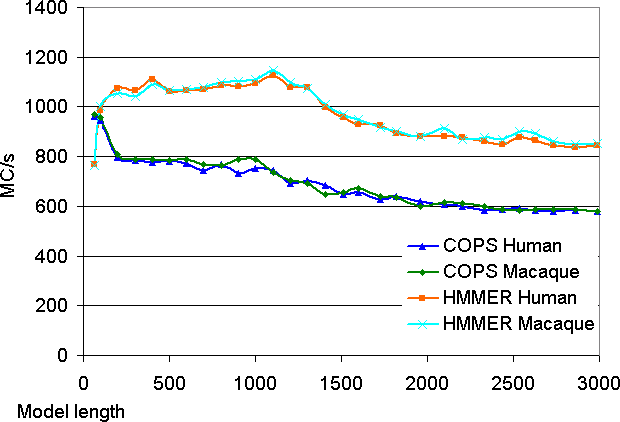
\includegraphics[scale=0.46]{graphics/initial-tags-runtimes.png}
		\caption[Speeds for the Inter-task vectorization on an Intel Xeon Nehalem] 
		{Speeds of the initial COPS and HMMER, with the Human and Macaque genomes, on an Intel Xeon Nehalem.}
		\label{initial-tags-runtimes}
    \end{minipage}
    \hspace{0.04\linewidth}
    \begin{minipage}{0.48\linewidth}
		\centering
		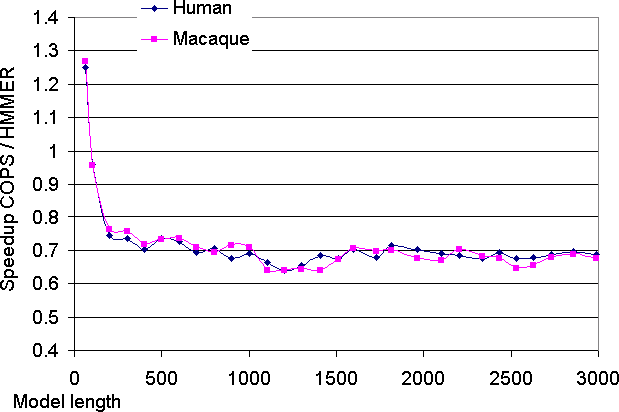
\includegraphics[scale=0.46]{graphics/initial-tags-speedups.png}
		\caption[Speedups for the Inter-task vectorization on an Intel Xeon Nehalem] 
		{Speedups of the initial COPS vs HMMER, with the Human and Macaque genomes, on an Intel Xeon Nehalem.}
		\label{initial-tags-speedups}
    \end{minipage}
\end{figure} 

\begin{figure}[h!]
    \begin{minipage}{0.48\linewidth}
		\centering
		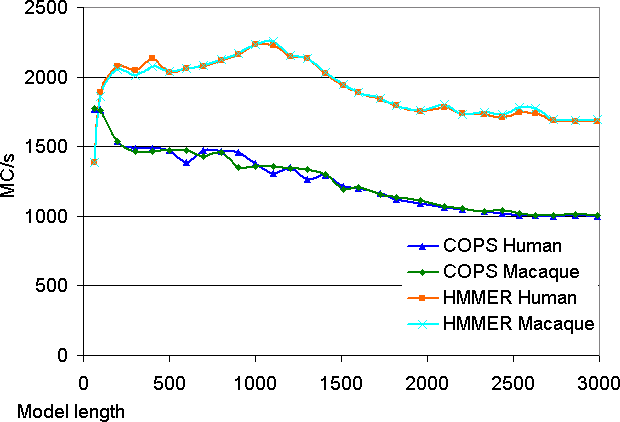
\includegraphics[scale=0.46]{graphics/initial-larissa-runtimes.png}
		\caption[Speeds for the Inter-task vectorization on an Intel i7 Sandy Bridge] 
		{Speeds of the initial COPS and HMMER, with the Human and Macaque genomes, on an Intel i7 Sandy Bridge.}
		\label{initial-larissa-runtimes}
    \end{minipage}
    \hspace{0.04\linewidth}
    \begin{minipage}{0.48\linewidth}
		\centering
		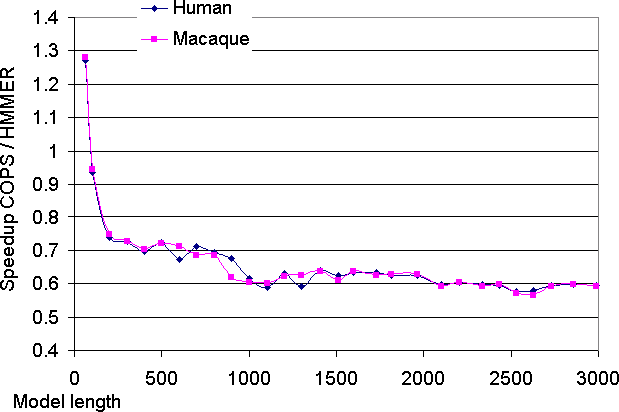
\includegraphics[scale=0.46]{graphics/initial-larissa-speedups.png}
		\caption[Speedups for the Inter-task vectorization on an Intel i7 Sandy Bridge]
		{Speedups of the initial COPS vs HMMER, with the Human and Macaque genomes, on an Intel i7 Sandy Bridge.}
		\label{initial-larissa-speedups}
    \end{minipage}
\end{figure} 

In this section, it is presented the results for the initial approach, based on Rognes' work, whose implementation was described in \sref{Rognes-based SSE Inter-task vectorization}. 

These results show that the original Rognes strategy is not able to surpass the performance of HMMER's ViterbiFilter, except in the case of the smaller models (lengths 60 and 100). From a length-100 model to a lengh-200, the performance of COPS drops drastically, as was discussed in \sref{Problems with First-level Cache Efficiency}.

On the Intel Sandy Bridge a substantial performance drop is also noticeable for larger models ($>$ length-1000). This second drop can also be explained by cache limitations, as it will disappear after normalizing the inner loop maximum memory use (see the later results of \sref{Results for the Model Partitioning}).

In very small models, length $<$ 80 bps, the performance of HMMER's striped version is particularly poor. This poor performance  was equally observed in the Smith-Waterman algorithm. It is caused by the substantial overhead of the Farrar's Lazy-F loop, which is run more frequently (relative to the size of the core computation load) when using very small models. The best results of Rognes' Smith-Waterman program against Farrar's were also found in these smaller lengths (for sequence queries).



\subsection{Results for the Inline loading of the Emission scores}
\label{Results for the Inline loading of the Emission scores}

\begin{figure}[H]
    \begin{minipage}{0.48\linewidth}
		\centering
		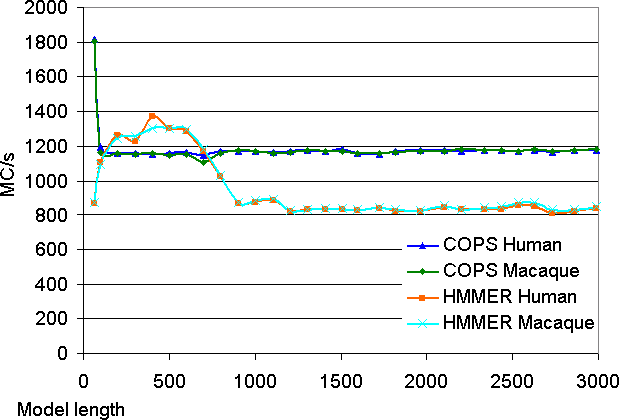
\includegraphics[scale=0.46]{graphics/inlined-aleph-runtimes.png}
		\caption[Speeds of COPS with Inlined Loading and HMMER on an AMD Opteron Bulldozer] 
		{Speeds of COPS with Inlined Loading and HMMER, Human and Macaque genomes, on an AMD Opteron Bulldozer.}
		\label{inlined-aleph-runtimes}
    \end{minipage}
    \hspace{0.04\linewidth}
    \begin{minipage}{0.48\linewidth}
		\centering
		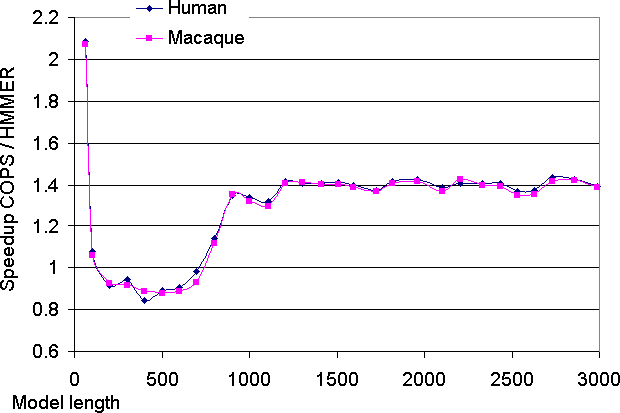
\includegraphics[scale=0.46]{graphics/inlined-aleph-speedups.png}
		\caption[Speedups of COPS with Inlined Loading vs HMMER on an AMD Opteron Bulldozer] 
		{Speedups of COPS with Inlined Loading vs HMMER, Human and Macaque genomes, on an AMD Opteron Bulldozer.}
		\label{inlined-aleph-speedups}
    \end{minipage}
\end{figure} 

\begin{figure}[H]
    \begin{minipage}{0.48\linewidth}
		\centering
		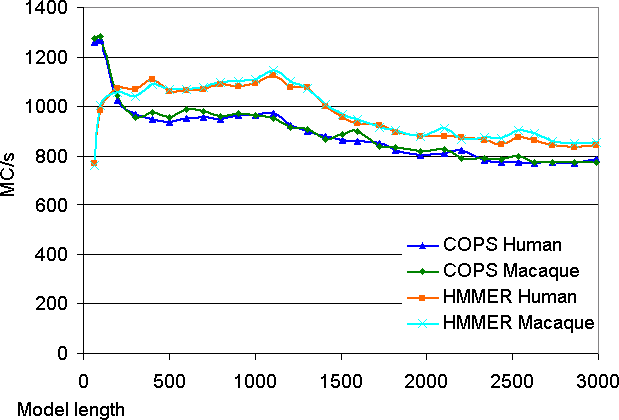
\includegraphics[scale=0.46]{graphics/inlined-tags-runtimes.png}
		\caption[Speeds of COPS with Inlined Loading and HMMER on an Intel Xeon Nehalem] 
		{Speeds of COPS with Inlined Loading and HMMER, Human and Macaque genomes, on an Intel Xeon Nehalem.}
		\label{inlined-tags-runtimes}
    \end{minipage}
    \hspace{0.04\linewidth}
    \begin{minipage}{0.48\linewidth}
		\centering
		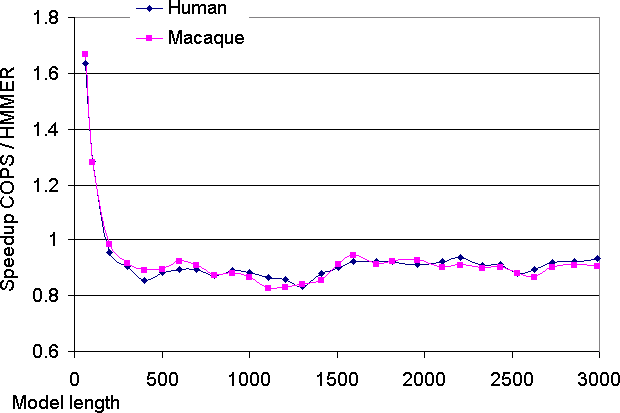
\includegraphics[scale=0.46]{graphics/inlined-tags-speedups.png}
		\caption[Speedups of COPS with Inlined Loading vs HMMER on an Intel Xeon Nehalem] 
		{Speedups of COPS with Inlined Loading vs HMMER, Human and Macaque genomes, on an Intel Xeon Nehalem.}
		\label{inlined-tags-speedups}
    \end{minipage}
\end{figure} 

In this section, Figures 5.7 to 5.12 present the results for the COPS version with the improvement of the loading and arrangement of Emission scores, by inlining the unpack operations in the inner loop. The development of this alternative Inline method was described in \sref{Loading of Emission Scores}. 

With this optimization, there is a general substantial performance boost, between 30\% and 40\% depending on the test machine (see Figures 5.13, 5.14 and 5.15). After this improvement, our COPS tool was able to beat HMMER on some machines (i.e. the AMD Opteron). Still, the performance dependency on model length remained mostly the same. The poor performance of HMMER in the smaller models, and the consequent higher speedup of COPS vs HMMER, remains also unchanged.

\clearpage

\begin{figure}[H]
    \begin{minipage}{0.48\linewidth}
		\centering
		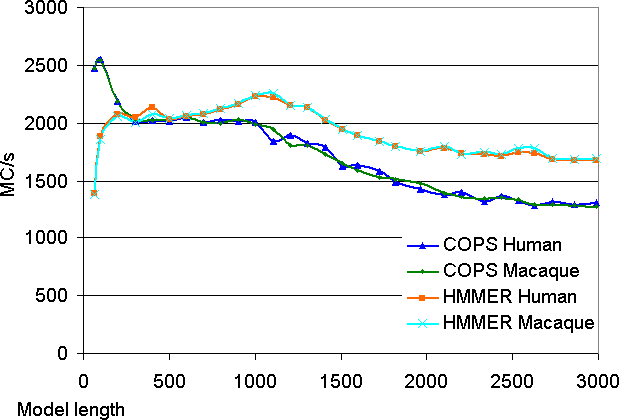
\includegraphics[scale=0.46]{graphics/inlined-larissa-runtimes.png}
		\caption[Speeds of COPS with Inlined Loading and HMMER on an Intel i7 Sandy Bridge] 
		{Speeds of COPS with Inlined Loading and HMMER, Human and Macaque genomes, on an Intel i7 Sandy Bridge.}
		\label{inlined-larissa-runtimes}
    \end{minipage}
    \hspace{0.04\linewidth}
    \begin{minipage}{0.48\linewidth}
		\centering
		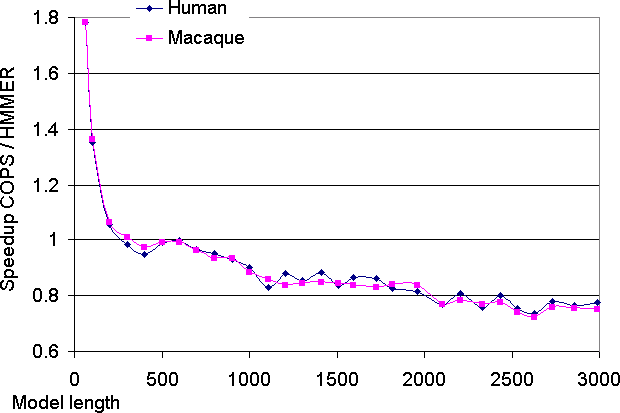
\includegraphics[scale=0.46]{graphics/inlined-larissa-speedups.png}
		\caption[Speedups of COPS with Inlined Loading and HMMER on an Intel i7 Sandy Bridge]
		{Speedups of COPS with Inlined Loading vs HMMER, Human and Macaque genomes, on an Intel i7 Sandy Bridge.}
		\label{inlined-larissa-speedups}
    \end{minipage}
\end{figure} 

\begin{figure}[H]
	\centering
	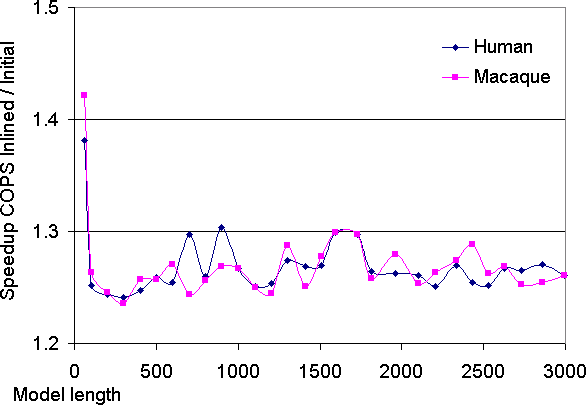
\includegraphics[scale=0.48]{graphics/inlined-cmp-aleph.png}
	\caption[Speedups of Inlined COPS vs Initial COPS on an Intel i7 Sandy Bridge] 
	{Speedups of COPS with Inlined Loading vs Initial COPS, Human and Macaque genomes, on an Intel i7 Sandy Bridge.}
	\label{inlined-cmp-aleph}
\end{figure} 

\begin{figure}[H]
    \begin{minipage}{0.48\linewidth}
		\centering
		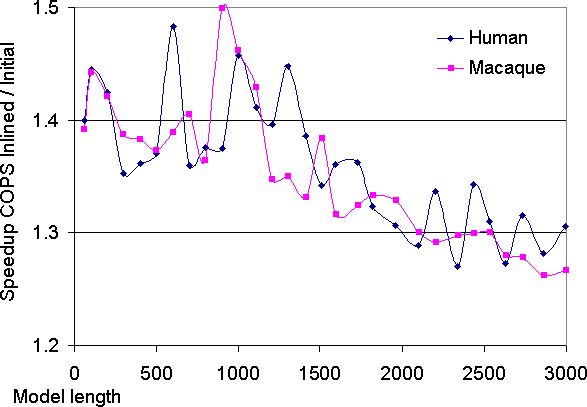
\includegraphics[scale=0.48]{graphics/inlined-cmp-larissa.png}
		\caption[Speedups of Inlined COPS vs Initial COPS on an Intel i7 Sandy Bridge] 
		{Speeds of COPS with Inlined Loading vs Initial COPS, Human and Macaque genomes, on an Intel i7 Sandy Bridge.}
		\label{inlined-cmp-larissa}
    \end{minipage}
    \hspace{0.04\linewidth}
    \begin{minipage}{0.48\linewidth}
		\centering
		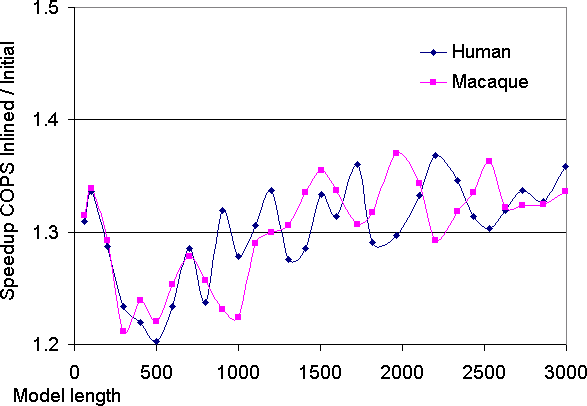
\includegraphics[scale=0.48]{graphics/inlined-cmp-tags.png}
		\caption[Speedups of Inlined COPS vs Initial COPS on an Intel i7 Sandy Bridge]
		{Speedups of COPS with Inlined Loading vs Initial COPS, Human and Macaque genomes, on an Intel i7 Sandy Bridge.}
		\label{inlined-cmp-tags}
    \end{minipage}
\end{figure} 





\subsection{Results for the Model Partitioning}
\label{Results for the Model Partitioning}

\begin{figure}[H]
    \begin{minipage}{0.48\linewidth}
		\centering
		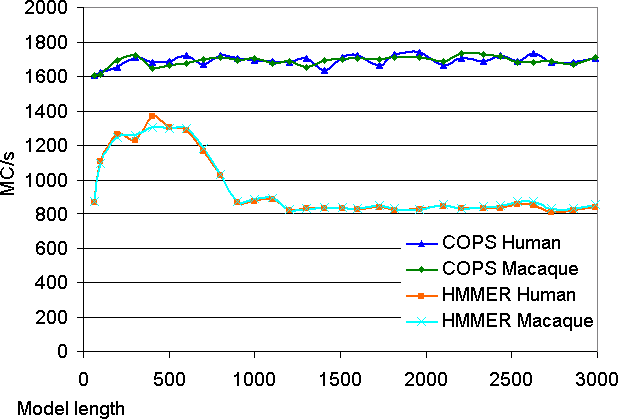
\includegraphics[scale=0.46]{graphics/partitions-aleph-runtimes.png}
		\caption[Speeds for the Inter-task vectorization on an AMD Opteron Bulldozer] 
		{Speeds of COPS after Partitioning and HMMER, with the Human and Macaque genomes, on an AMD Opteron Bulldozer.}
		\label{partitions-aleph-runtimes}
    \end{minipage}
    \hspace{0.04\linewidth}
    \begin{minipage}{0.48\linewidth}
		\centering
		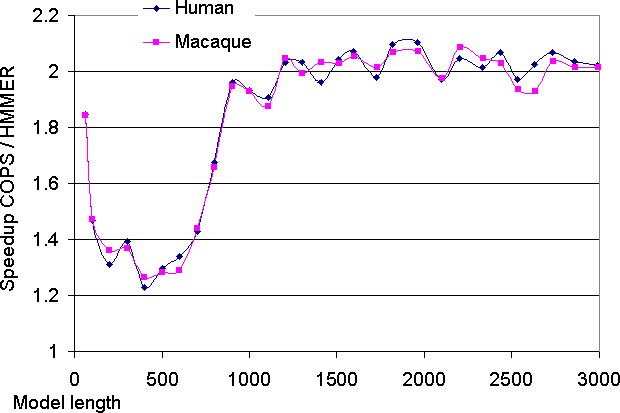
\includegraphics[scale=0.46]{graphics/partitions-aleph-speedups.png}
		\caption[Speedups for the Inter-task vectorization on an AMD Opteron Bulldozer] 
		{Speedups of COPS after Partitioning vs HMMER, with the Human and Macaque genomes, on an AMD Opteron Bulldozer.}
		\label{partitions-aleph-speedups}
    \end{minipage}
\end{figure} 

\begin{figure}[H]
    \begin{minipage}{0.48\linewidth}
		\centering
		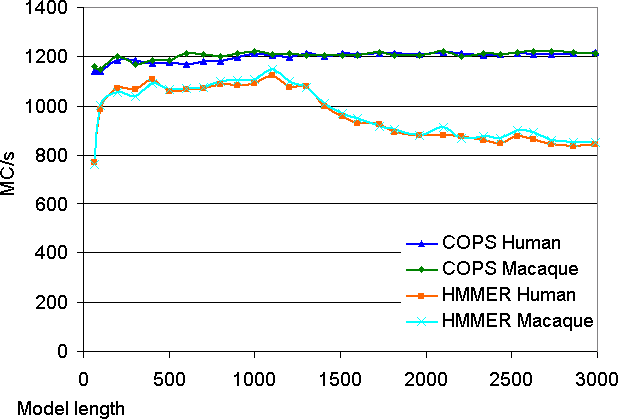
\includegraphics[scale=0.46]{graphics/partitions-tags-runtimes.png}
		\caption[Speeds for the Inter-task vectorization on an Intel Xeon Nehalem] 
		{Speeds of COPS after Partitioning and HMMER, with the Human and Macaque genomes, on an Intel Xeon Nehalem.}
		\label{partitions-tags-runtimes}
    \end{minipage}
    \hspace{0.04\linewidth}
    \begin{minipage}{0.48\linewidth}
		\centering
		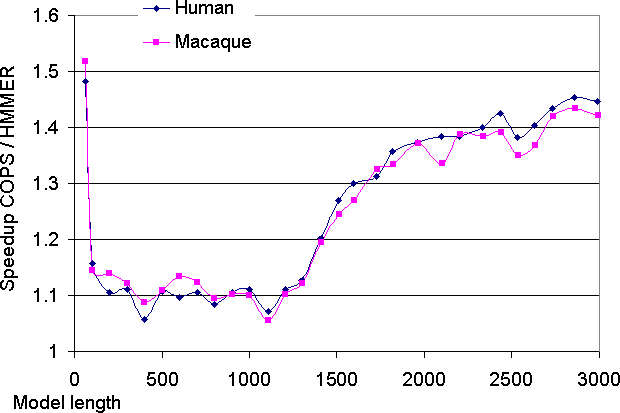
\includegraphics[scale=0.46]{graphics/partitions-tags-speedups.png}
		\caption[Speedups for the Inter-task vectorization on an Intel Xeon Nehalem] 
		{Speedups of COPS after Partitioning vs HMMER, with the Human and Macaque genomes, on an Intel Xeon Nehalem.}
		\label{partitions-tags-speedups}
    \end{minipage}
\end{figure} 


These are the results for the COPS version after partitioning the HMM model, which has been described in \sref{Model Partitioning to improve the L1 cache utilization}. This evaluated version includes the inline loading of Emission scores.

With model partitioning, the L1 cache size limitation is overcome, and therefore the performance drop from length-100 models to 200-length models, that was evident in the earlier results, disappears. The performance of this version of COPS remains constant with increasing model lengths, in all test machines. 

In particular, this improvement is observed equally in Intel's 32KB L1D cache machines, and in AMD's Opterons with a 16KB L1D cache (see \autoref{partitions-aleph-runtimes}). The optimal partition length was specifically tuned for each test machine (namely, a length of 112-120 for Intel's 32KB caches, and 48 for AMD's 16KB caches). For larger models (length $>$ 1000), COPS is able to beat HMMER on all machines, achieving a speedup ranging from 1.5x on the Intel machines, to 2x on the AMD.

\begin{figure}[h!]
    \begin{minipage}{0.48\linewidth}
		\centering
		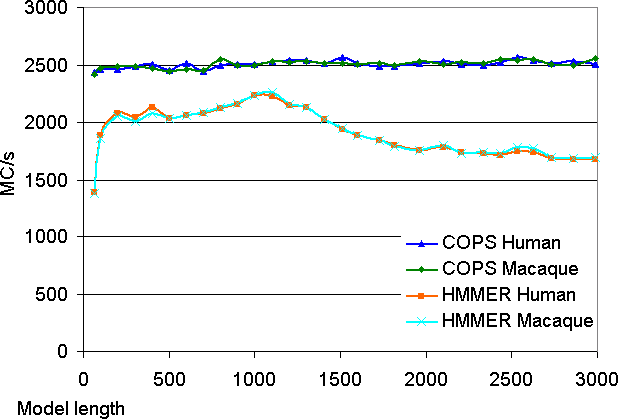
\includegraphics[scale=0.46]{graphics/partitions-larissa-runtimes.png}
		\caption[Speeds for the Inter-task vectorization on an Intel i7 Sandy Bridge] 
		{Speeds of COPS after Partitioning and HMMER, with the Human and Macaque genomes, on an Intel i7 Sandy Bridge.}
		\label{partitions-larissa-runtimes}
    \end{minipage}
    \hspace{0.04\linewidth}
    \begin{minipage}{0.48\linewidth}
		\centering
		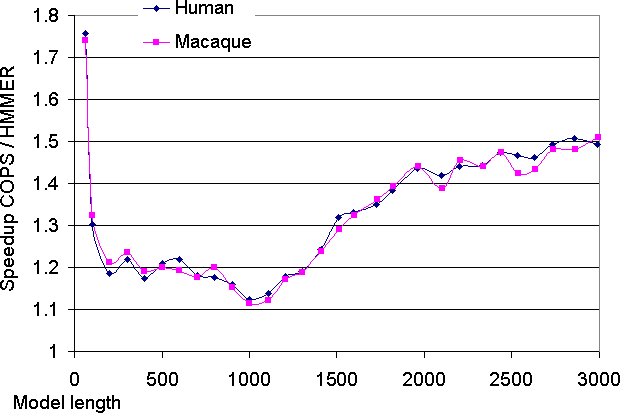
\includegraphics[scale=0.46]{graphics/partitions-larissa-speedups.png}
		\caption[Speedups for the Inter-task vectorization on an Intel i7 Sandy Bridge]
		{Speedups of COPS after Partitioning vs HMMER, with the Human and Macaque genomes, on an Intel i7 Sandy Bridge.}
		\label{partitions-larissa-speedups}
    \end{minipage}
\end{figure} 

It can be seen in the results that the speedup of COPS vs. HMMER still drops considerably from the smaller M-60 model to the next length-100 model. As referenced before, this drop is explained by the poor showing of HMMER's Viterbifilter in the smaller model. HMMER's striped version executes the \emph{Lazy-F} loop more frequently when the sequence stride is shorter, having a shorter available span to nullify the $F$ dependencies ($D$ for HMMs), and this happens when the model is smaller. Therefore the speedup drop vs. HMMER from the length-60 to the length-100 model is not caused by an efficiency decrease of our version, but by an increase in HMMER. The performance of COPS remains mostly constant in these smaller models, as can be seen in the processing speed graphic.

Therefore, for short models ($<$ 100 bps), COPS achieves a considerable 1.7-fold speedup vs HMMER. For medium-length models (between 200 and 500 bps on 16KB-L1D machines, and up to $\sim$1000 on 32KB-L1D machines), HMMER's implementation is competitive against COPS, reducing our speedup to about 1.2-fold. These are the model lengths wherein the striped version does not exceed the size of the innermost data cache. 

Still, the speedups for short models have not been as high as the ones reported by Rognes for Smith-Waterman. Many reasons may justify this, such as Rognes' aggressive assembly optimizations, and the unavoidable differences between the Viterbi and Smith-Waterman algorithms. One significant cause in our view is the overall higher memory requirements of Viterbi. A inter-task approach is bound to required significantly more memory that an intra-task vectorization, 8-fold for some of the data.

For longer models, from 500 bps or 1000 bps depending on the L1D size, it can be observed that the performance of HMMER quickly deteriorates as the model's length increases, and the memory requirements of the standard Farrar approach reach the maximum that the innermost caches can provide. In contrast, COPS is able to consistently maintain the same performance with increasingly long models, thus achieving a 2-fold speedup on AMD's, and 1.5-fold on Intel's, against HMMER's striped implementation.


The optimized serial benchmark managed a meager result of 228 MC/s on the Core i7, 201 MC/s on the Intel Xeon, and 153MC/s on the AMD, for every model. So, the overall speedup over the non-parallelized code is 11x in the Core i7, 8x on the Intel Xeon, and 8.5x on the AMD.




\subsection{Results for the Wave-Front Multi-threading}
\label{Results for the Wave-Front Multi-threading}

The graphics with the results for the multi-threaded COPS are presented in Appendix A. This version uses a multi-threaded wave-front pattern in the partitions (described in \sref{Multi-threading the partitions}). The evaluation was conducted with an increasing number of threads, 1, 2, 4, 6, and 8 for the 8-core machines.

HMMER's ViterbiFilter is run with independent tasks per thread, in a multi-threaded work pool. Therefore, it is strongly expected that it achieves a quasi-linear speedup over the number of threads, since each thread proceeds independent of the others. The only synchronization point is the access to the work queue, to fetch each new sequence. This synchronization cost is very light - it was measured by comparing against a static work decomposition with same-length sequences (which does not require synchronization primitives), and found to be practically unnoticeable.

The experimental results show that HMMER's Intra-task implementation is able to maintain a linear speedup over the number of threads/scores. This is was the expected outcome, since it is processing each alignment task independently, and there are no inter-thread dependencies (except for the shared work pool).

In the case of COPS, the results show a clear sub-linear speedup, with a considerable drop in the added speed per core, as the number of cores increase. This was also an expected outcome, since there is substantial communication between the threads processing the partitions. Still, other causes may account for some of the lost processing speed. These will be discussed in \sref{Limitations of Wave-Front Multi-threading}. But first, in the next section, the program will be analyzed through Karp-Flatt metric, estimating the serial fraction of the developed program, i.e., the non-parallelized fraction.



\subsection{Evaluation of the experimental serial fraction by Karp-Flatt's Metric}

Karp and Flatt \cite{karpflatt} proposed a metric to measure the portion of a program that is inherently sequential and cannot (or has not) been parallelized - the Experimentally-determined serial fraction ($e$). The metric estimates the value of $e$ by the following formula:

$$ e = \frac{ \displaystyle \frac{1}{Speedup} - \frac{1}{p} } { \displaystyle 1 - \frac{1}{p} } $$

The values derived with this metric from the tests conducted are shown in the graphics below.
%Only the results for the Human genome are presented because the values for the Macaque genome are very close.

\begin{figure}[h!]
    \begin{minipage}{0.48\linewidth}
		\centering
		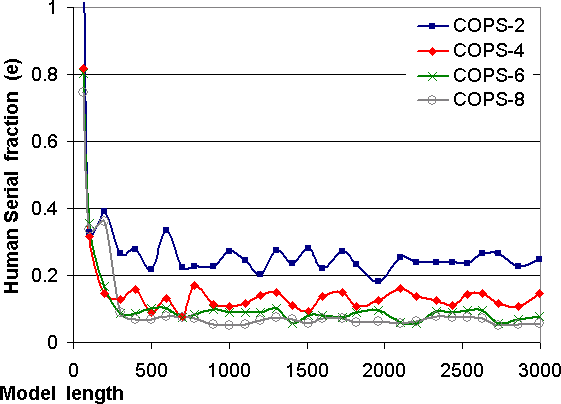
\includegraphics[scale=0.46]{graphics/karp-flatt-aleph-human.png}
		\caption[Serial fraction on AMD Opteron Bulldozer, Human] {Experimental serial fraction using Karp-Flatt's metric, for the AMD Opteron Bulldozer tests with Human DNA.}
	\label{karp-flatt-aleph-human}
    \end{minipage}
    \hspace{0.04\linewidth}
    \begin{minipage}{0.48\linewidth}
		\centering
		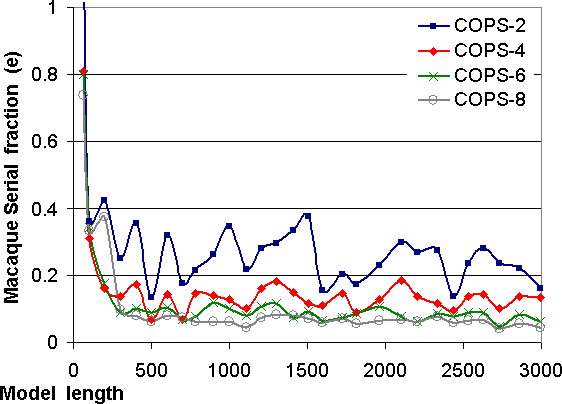
\includegraphics[scale=0.46]{graphics/karp-flatt-aleph-macaque.png}
		\caption[Serial fraction on AMD Opteron Bulldozer, Macaque] {Experimental serial fraction using Karp-Flatt's metric, for the AMD Opteron Bulldozer tests with Macaque DNA.}
	\label{karp-flatt-aleph-macaque}
    \end{minipage}
\end{figure} 

\begin{figure}[h!]
    \begin{minipage}{0.48\linewidth}
		\centering
		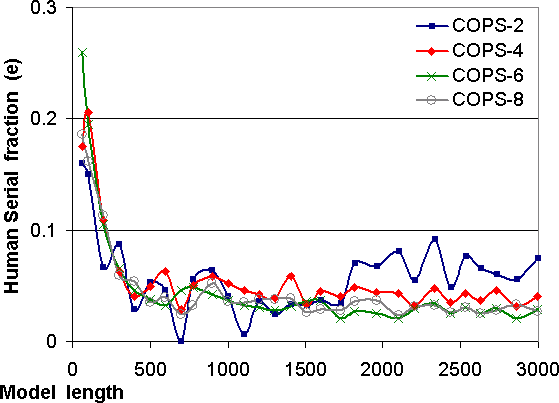
\includegraphics[scale=0.46]{graphics/karp-flatt-tags-human.png}
		\caption[Serial fraction on Intel Xeon Nehalem, Human] {Experimental serial fraction using Karp-Flatt's metric, for the Intel Xeon Nehalem tests with Human DNA.}
		\label{karp-flatt-tags-human}
    \end{minipage}
    \hspace{0.04\linewidth}
    \begin{minipage}{0.48\linewidth}
		\centering
		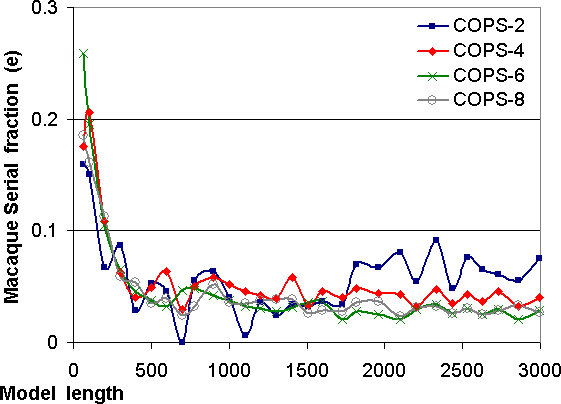
\includegraphics[scale=0.46]{graphics/karp-flatt-tags-macaque.png}
		\caption[Serial fraction on Intel Xeon Nehalem, Macaque] {Experimental serial fraction using Karp-Flatt's metric, for the Intel Xeon Nehalem tests with Macaque DNA.}
		\label{karp-flatt-tags-macaque}
	\end{minipage}
\end{figure} 

\begin{figure}[h!]
    \begin{minipage}{0.48\linewidth}
		\centering
		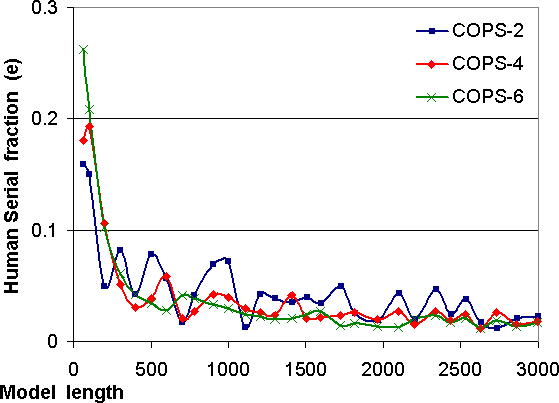
\includegraphics[scale=0.48]{graphics/karp-flatt-larissa-human.png}
		\caption[Serial fraction on Intel i7 Sandy Bridge, Human] {Experimental serial fraction using Karp-Flatt's metric, for the Intel i7 Sandy Bridge tests with Human DNA.}
		\label{karp-flatt-larissa-human}
    \end{minipage}
    \hspace{0.04\linewidth}
    \begin{minipage}{0.48\linewidth}
		\centering
		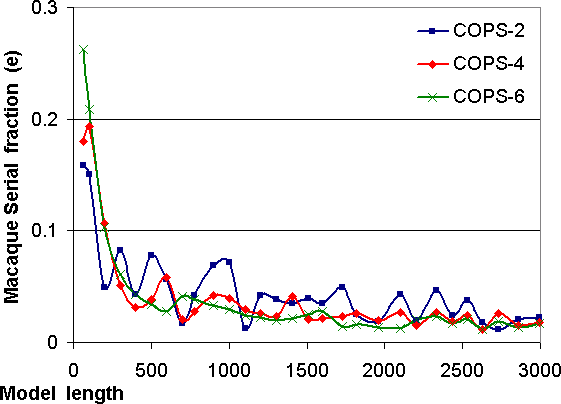
\includegraphics[scale=0.48]{graphics/karp-flatt-larissa-macaque.png}
		\caption[Serial fraction on Intel i7 Sandy Bridge, Macaque] {Experimental serial fraction using Karp-Flatt's metric, for the Intel i7 Sandy Bridge tests with Macaque DNA.}
		\label{karp-flatt-larissa-macaque}
	\end{minipage}
\end{figure} 

In general, the serial fraction consistently decreases with the number of threads, in all models, which substantiate the assumption that most of the performance loss is due to the parallel overhead, instead of non-parallelized code. However, there is one exception: in the smaller models (length $<=$ 200), the serial fraction is both considerable higher (indicating a worse parallelization), and it changes little with the number of threads. This result suggests that there is a substantial non-parallelized computation load in these models. That can be explained by the difficulty in finding an optimal work division between partitions and threads, as will be further discussed in the next section.

Another interesting point of note are the wide variations in the serial fraction metric along model lengths, reflecting an efficiency of multi-threading that depends on the specific model length. Some model lengths allow for a perfect work decomposition between partitions and threads, while others do not, and leave some unbalanced workloads. This will also be further discussed in the next section. 

The parallelization had a lower speedup per added thread on the AMD machine than it did on the Intel machines. The different internal architectures of the two different processor families is a likely culprit for this anomaly, since it was found that even a set of independent, non-communicating processes became considerably slower when running concurrently. Additionally, the AMD machine was deployed in a NUMA topology, with a distributed shared memory. The configuration of the DSM seriously hindered any concurrent contention for resources, even among independent processes running on the same NUMA node. 




\subsubsection{Limitations of Wave-Front Multi-threading} 
\label{Limitations of Wave-Front Multi-threading} 

A multi-threading parallelization of the Model partitions, using a wave-front pattern, suffers from some problems that affect its efficiency, and lead to a sub-linear and decreasing parallel speedup:

\begin{itemize}

\item \textbf{Communication overhead}

There are two communication instances between the threads: 
\begin{itemize}[nolistsep]
\item a synchronization point on the flags' arrays, each one shared by only two threads;
\item a data transfer point on partition barriers, which is only accessed before (for writes) and after (for reads) the synchronization point.
\end{itemize}

There is therefore no real contention on the data transfer point, since it is guaranteed to be accessed by only one thread at any given time. The synchronization point suffers some contention from its two owner threads, and the wait cycles when one thread is blocked waiting for the other lead to a non-negligible fraction of thread idle time.


\item \textbf{Start and end delays of the wave-front pattern}

The wave-front pattern entails some unavoidable wait cycles in the start and end of the alignment. Each thread must wait that the previous thread finished the previous partition column, and as a result there is a incremental delay in the beginning, wherein the necessary delay of each thread increases by one work chunk (i.e. one partition column) for each added thread. In the ending of the alignment, the threads that started earlier have to wait for the ones lagging behind, with wait periods in the reserve order.


\item \textbf{Unbalanced work division}

The perfect work division is an even division of the partitions by the threads, and of the model length by the partition length. However it is not always possible to find such a division, especially when the number of threads is higher. The thread work load will become unbalanced in two cases:
\begin{itemize}[nolistsep]
\item When the partitions cannot be evenly distributed by the threads, some thread(s) will get less partitions to process, and will have to wait on the others to finish;
\item When the model length is not evenly divisible by the partition length, the last thread will have less work than the others, and thus will also have to wait. This last unbalanced partition represents a smaller waste than the unbalanced number of partitions, which force thread(s) to wait for the computation period of a whole partition.
\end{itemize}

\item \textbf{Very short partition lengths}

When using partitions that are too small, the various overheads (initialization, termination, synchronization, wave-front delays,  unbalancing idle times, etc) are a large fraction of the overall runtime, due to the corresponding core computation load that has been reduced by the short partition length. These partition lengths should be avoided, but for very small models it may not be possible.

%\item a thread main tem trabalho adicional a preparar a inicializacao, e a extrair os resultados no final => 0.1segs em 84 (fracao)

\end{itemize}
	
The quite noticeable lower speedup per added thread in the smaller models is explained by the uneven load balancing between the threads (some threads have less partitions to compute) and by the heavier overheads when using shorter partition lengths. As more cores are added, the speedup of the wave-front COPS vs HMMER decreases considerably in the smaller models, because the inter-task trivial multi-threading implemented for HMMER's ViterbiFilter does not have these load balancing problems in the test databases (i.e. databases with many sequences).

Conversely, the speedup per added core is higher in the longer models, since they have a better load balancing and a smaller overhead from the longer partitions. Therefore, to effectively exploit the multi-threaded wave-front pattern for a high number of threads (i.e. 8 threads), the application's models should be sufficiently large, in order to reduce the incurred overheads with a close-to-maximum partition length, and achieve an even distribution of partitions among threads.



%\cleardoublepage
\clearpage





